\documentclass[mathserif]{beamer}
\usepackage{amsmath}
\usepackage{multicol}
\usepackage{tikz} % for label positions
\usepackage{amsmath}
\usetikzlibrary{arrows.meta, positioning, shapes}


% \usetikzlibrary{graphs}

\definecolor{myorange}{RGB}{129,1,0}
\setbeamercolor{structure}{fg=myorange}
\setbeamercolor{title}{fg=myorange}


\title{\textbf{Seven Bridges of K\"{o}nigsberg}}
\subtitle{}
\author{Akshay Sanjeev Keloth\\ \small Institute of Mathematical Sciences, Chennai}

\begin{document}

\begin{frame}
\maketitle
\end{frame}

\begin{frame}{K\"{o}nigsberg aka Kalinigrad}
    \begin{figure}
        \centering
        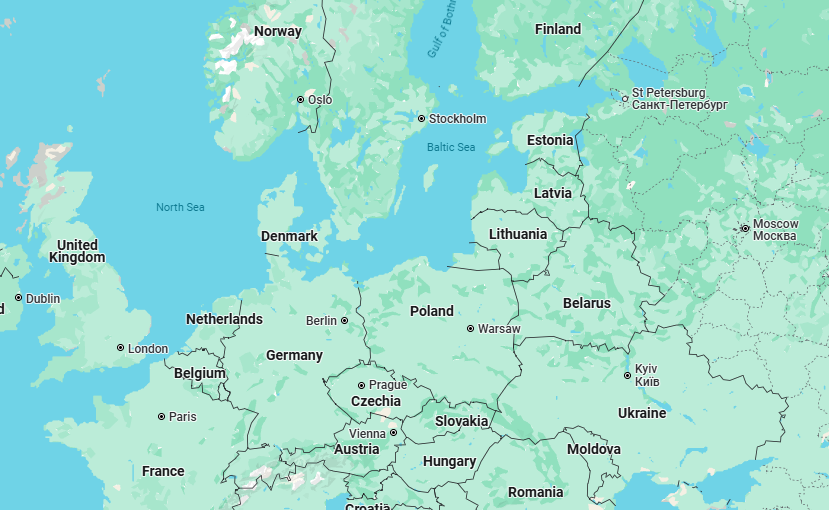
\includegraphics[scale=.5]{bigmap.png}
        \caption{(Source: Google Maps)}
    \end{figure}
\end{frame}



\begin{frame}{The Probelm}
    \begin{figure}
        \centering
        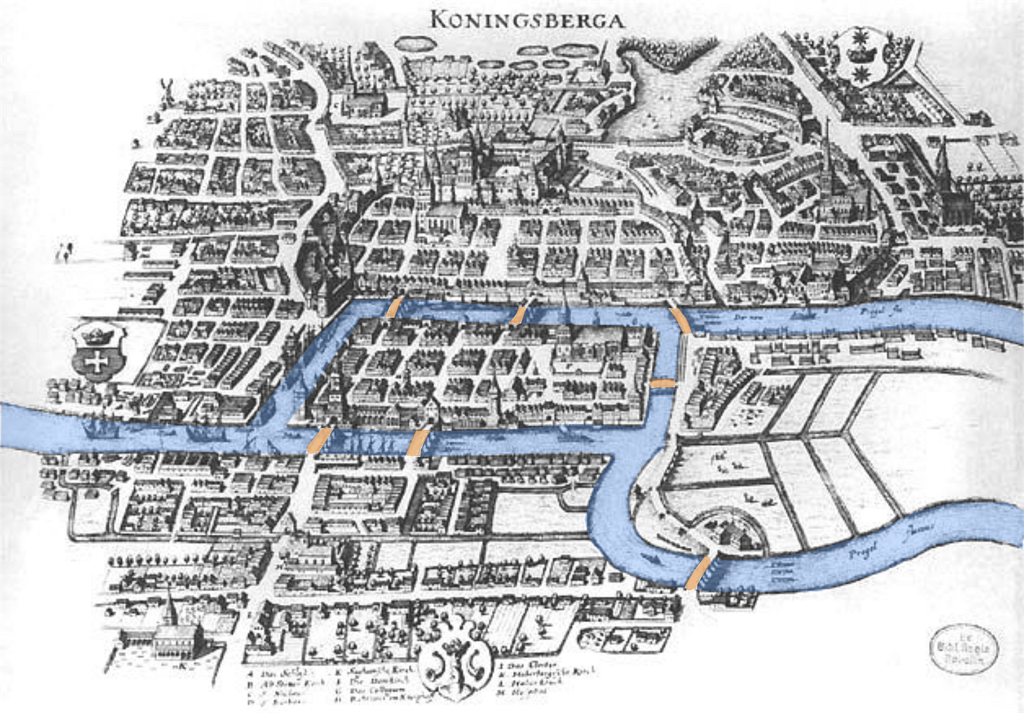
\includegraphics[scale=.25]{map1.png}
        \caption{(Source: Merian-Erben, Wikimedia Commons)}
    \end{figure} 
\end{frame}

\begin{frame}{Current situation}
    \begin{figure}
        \centering
        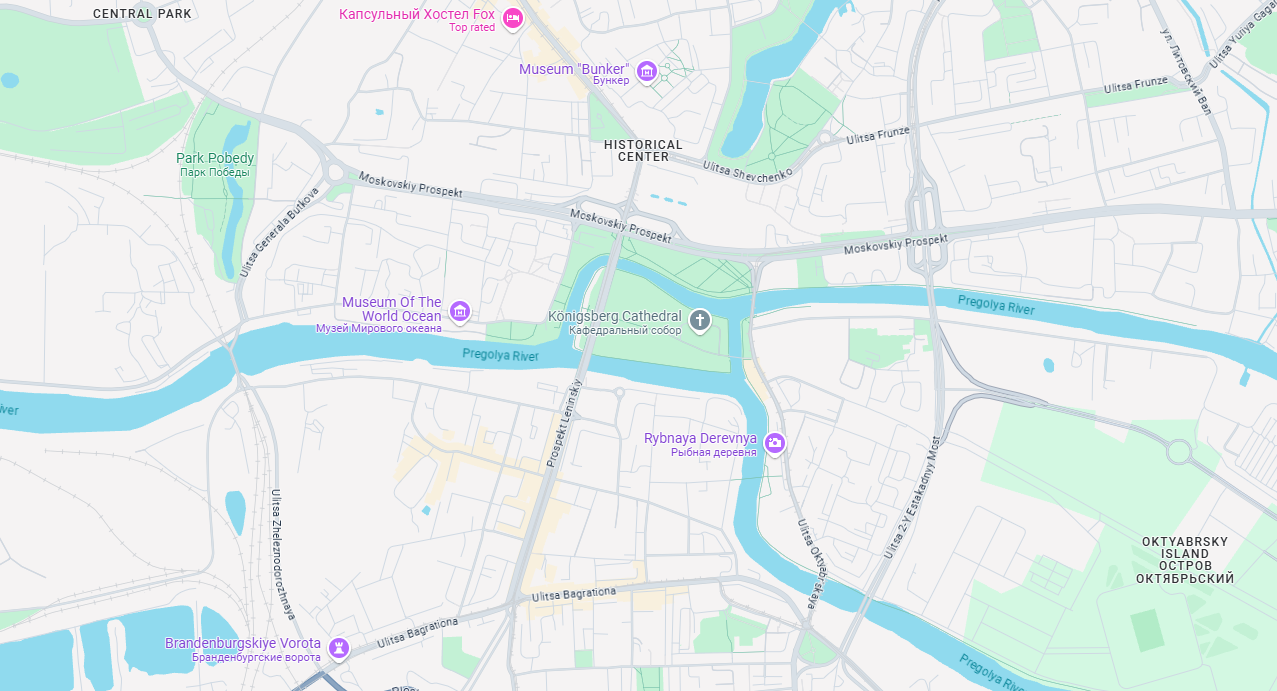
\includegraphics[scale=.3]{zoom.png}
        \caption{(Source: Google Maps)}
    \end{figure}
\end{frame}


\begin{frame}{A new problem!}
    \begin{figure}
        \centering
        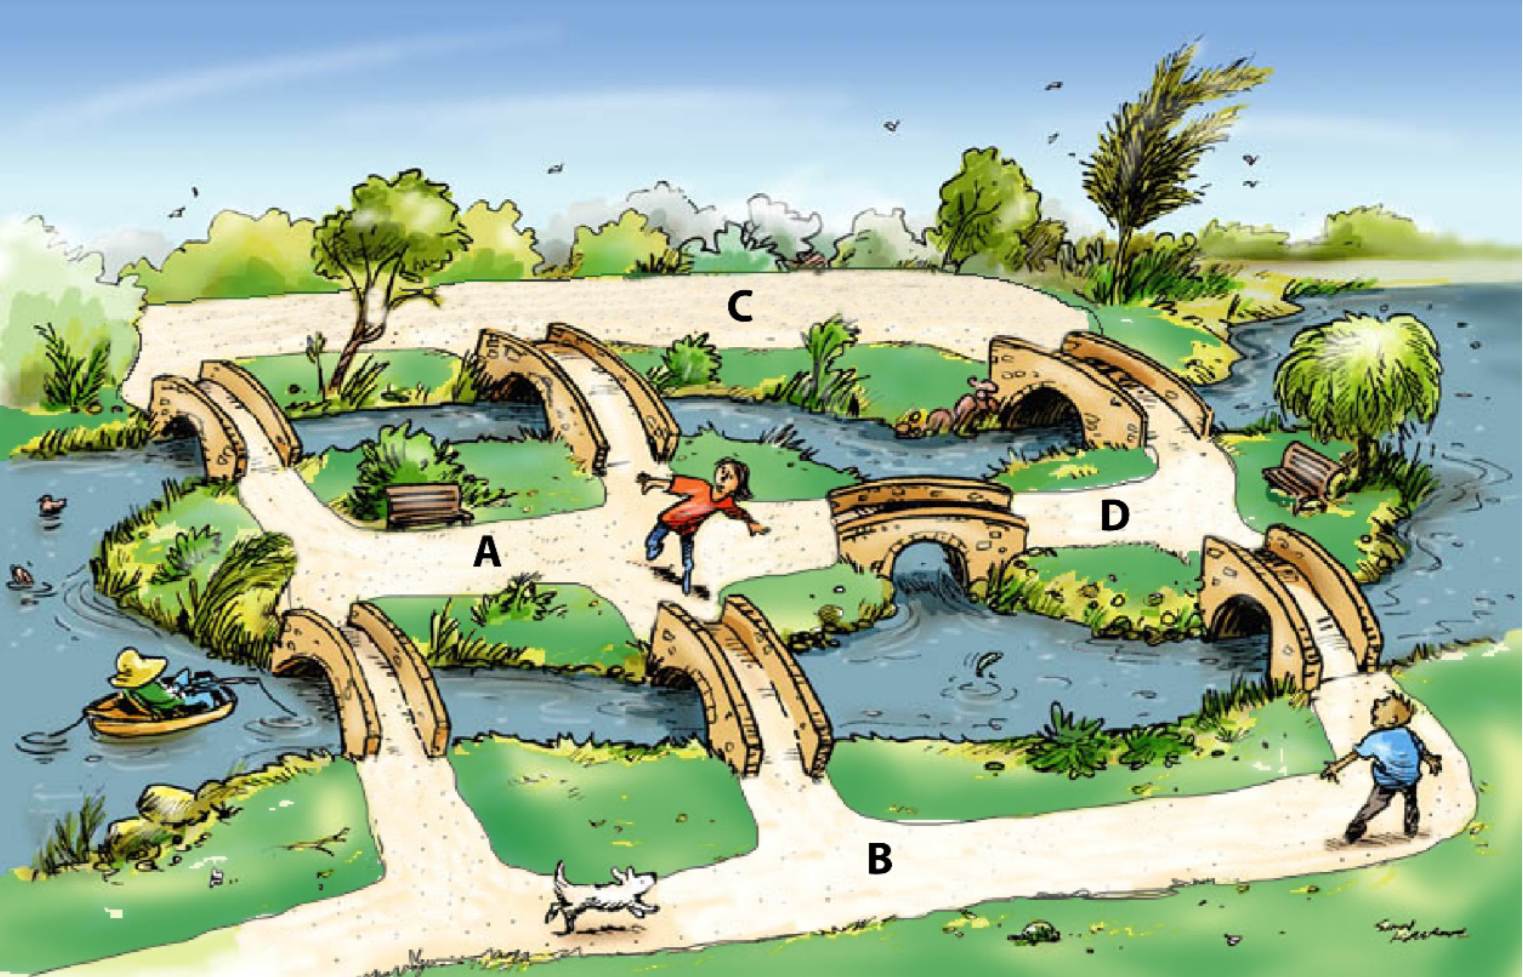
\includegraphics[scale=.25]{map2.png}
        % \caption{Source: Merian-Erben, Wikimedia Commons}
    \end{figure}
\end{frame}

\begin{frame}{Is it really?}
    \begin{enumerate}
        \item  Can you find the required path?
        \item  Is this picture same as the one you saw of K\"{o}nigsberg Bridges? 
        \item Can you try to simplify the picture?
    \end{enumerate}
    \end{frame}

% \begin{frame}
%     \begin{figure}
%         \centering
%         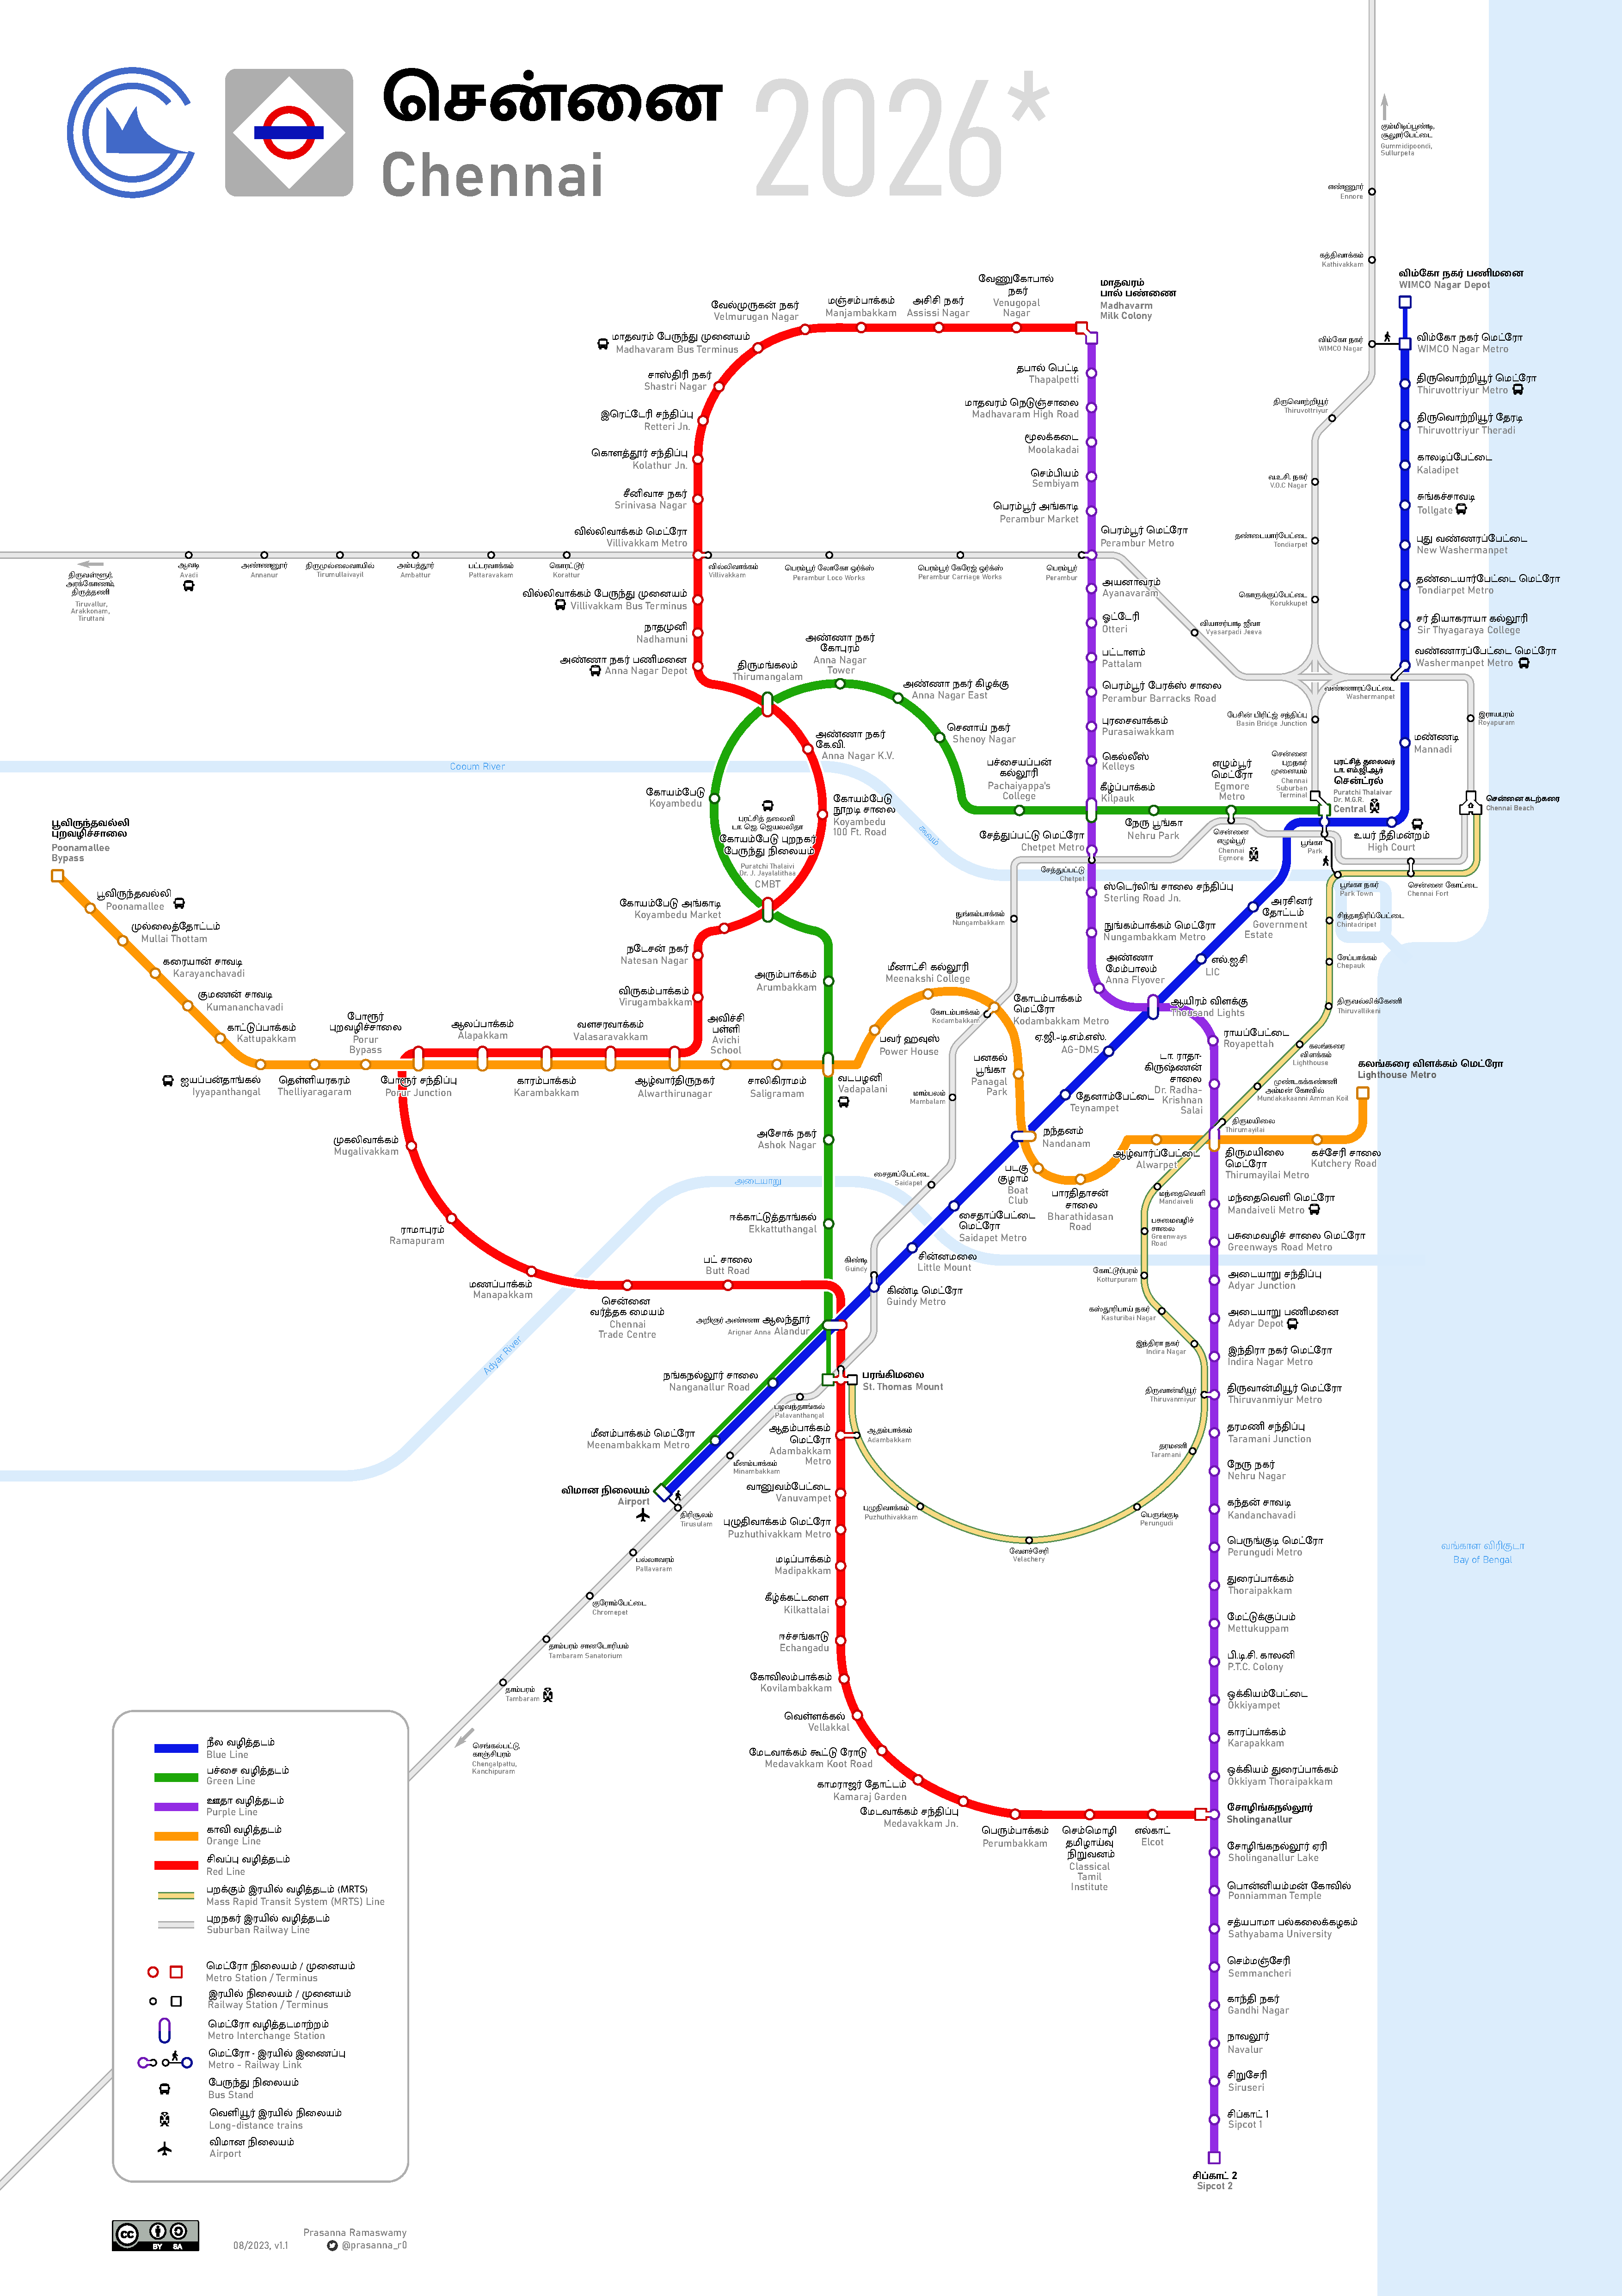
\includegraphics[scale=.1]{metromap.pdf}
%     \end{figure}
% \end{frame}


\begin{frame}{Another probelm!}
    Can you draw this picture without lifting the pencil?
    \vskip5mm
    \begin{figure}
    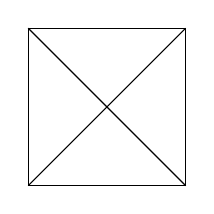
\begin{tikzpicture}
    % Draw square
    \draw (0,0) -- (2,0) -- (2,2) -- (0,2) -- cycle;
    % Draw diagonals
    \draw (0,0) -- (2,2);
    \draw (0,2) -- (2,0);
    \end{tikzpicture}
    \end{figure}
    \vskip5mm
    \pause 
    Is this somehow related to the K\"{o}nigsberg problem?
\end{frame}

\begin{frame}{A Graph}
    \centering
    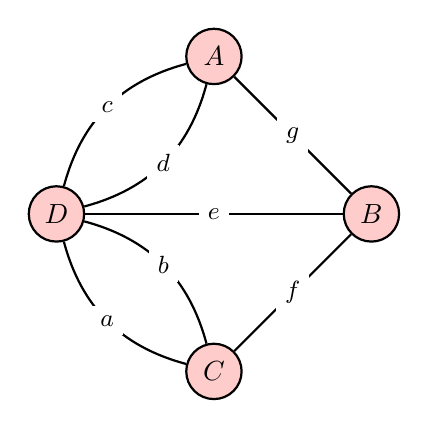
\begin{tikzpicture}[
    node style/.style={circle, draw=black, fill=red!20, minimum size=20pt, inner sep=2pt},
    % node/.style={circle, draw=black, fill=red!30, minimum size=20pt, inner sep=0pt},
    edgelabel/.style={midway, fill=white, font=\small},
    every path/.style={thick, black},
]

    % % Node
    \node[node style ] (A) at (0,4)  {$A$};
    \node[node style  ] (B) at (2,2) {$B$};    
    \node[node style  ] (C) at (0,0) {$C$};
    \node[node style  ] (D) at (-2,2){$D$};

    % Edges with labels
    \draw[bend left=30] (A) to node[edgelabel] {$d$} (D);
    \draw[bend right=30] (A) to node[edgelabel] {$c$} (D);

    \draw (A) -- node[edgelabel] {$g$} (B);
    \draw (D) -- node[edgelabel] {$e$} (B);

    \draw[bend left=30] (C) to node[edgelabel] {$a$} (D);
    \draw[bend right=30] (C) to node[edgelabel] {$b$} (D);

    \draw (C) -- node[edgelabel] {$f$} (B);

    \end{tikzpicture}

\pause
Now can you try to trace the lines without lifting your pencil?
\end{frame}

\begin{frame}{Graph Theory 101}
    A graph is made of a set of  points and lines connecting them. These 
points are called \textbf{nodes} or \textbf{vertices}. The lines are called
\textbf{edges}\footnote{The terminology is inconsistent between fields}.
Degree is the number of edges connected to a node. 
\centering \vskip5mm
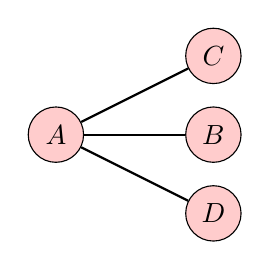
\begin{tikzpicture}[
    node style/.style={circle, draw=black, fill=red!20, minimum size=20pt, inner sep=2pt}
]
\node[node style] (A) at (0,0) {$A$};
\node[node style] (B) at (2,0) {$B$};
\node[node style] (C) at (2,1) {$C$};
\node[node style] (D) at (2,-1){$D$};

\draw[thick] (A) -- (B);
\draw[thick] (A) -- (C);
\draw[thick] (A) -- (D);
\end{tikzpicture}

\pause

\begin{align*}
    d(A) &= 3 \\
    d(p) &= 1, \qquad p = B, C, D
\end{align*} 

\end{frame}

\begin{frame}{Graph Theory 101}
    A graph is made of a set of  points and lines connecting them. These 
points are called \textbf{nodes} or \textbf{vertices}. The lines are called
\textbf{edges}\footnote{The terminology is inconsistent between fields}.
Degree is the number of edges connected to a node. 
    \centering
    \vskip5mm
    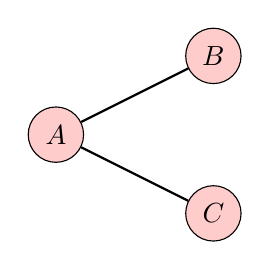
\begin{tikzpicture}[
    node style/.style={circle, draw=black, fill=red!20, minimum size=20pt, inner sep=2pt}
]
        \node[node style] (A) at (0, 0) {$A$};
        \node[node style] (B) at (2, 1) {$B$};
        \node[node style] (C) at (2, -1) {$C$};

        \draw[thick] (A) -- (B);
        \draw[thick] (A) -- (C);
    \end{tikzpicture}
    \begin{align*}
    d(A) &= 2 \\
    d(p) &= 1, \qquad p = B, C
\end{align*} 
\end{frame}


\begin{frame}{Find the degrees}
\begin{columns}
% Left column: Graph
\begin{column}{0.6\textwidth}
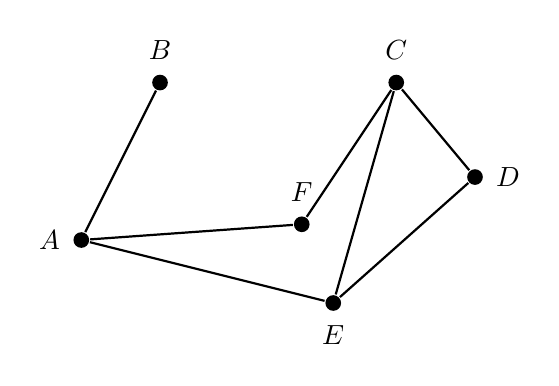
\begin{tikzpicture}[every node/.style={circle, fill=black, inner sep=2pt}, 
                    every path/.style={thick}]

% Nodes
\node[label=left:$A$]  (A) at (0,0)   {};
\node[label=above:$B$] (B) at (1,2)   {};
\node[label=above:$C$] (C) at (4,2)   {};
\node[label=right:$D$] (D) at (5,0.8) {};
\node[label=below:$E$] (E) at (3.2,-0.8) {};
\node[label=above:$F$] (F) at (2.8,.2)   {};

% Edges
\draw (A) -- (B);
\draw (A) -- (F);
\draw (A) -- (E);
\draw (F) -- (C);
\draw (C) -- (E);
\draw (C) -- (D);
\draw (D) -- (E);

\end{tikzpicture}
\end{column}
\pause 
% Right column: Degree Table
\begin{column}{0.4\textwidth}
\begin{tabular}{|c|c|}
\hline
\textbf{Node} & \textbf{Degree} \\
\hline
$A$ & 3 \\
$B$ & 1 \\
$C$ & 3 \\
$D$ & 2 \\
$E$ & 3 \\
$F$ & 2 \\
\hline
\end{tabular}
\end{column}
\end{columns}
\pause
\vskip10mm
Draw a graph and try to work out the degrees! 


\end{frame}


\begin{frame}{Some more examples}
\centering
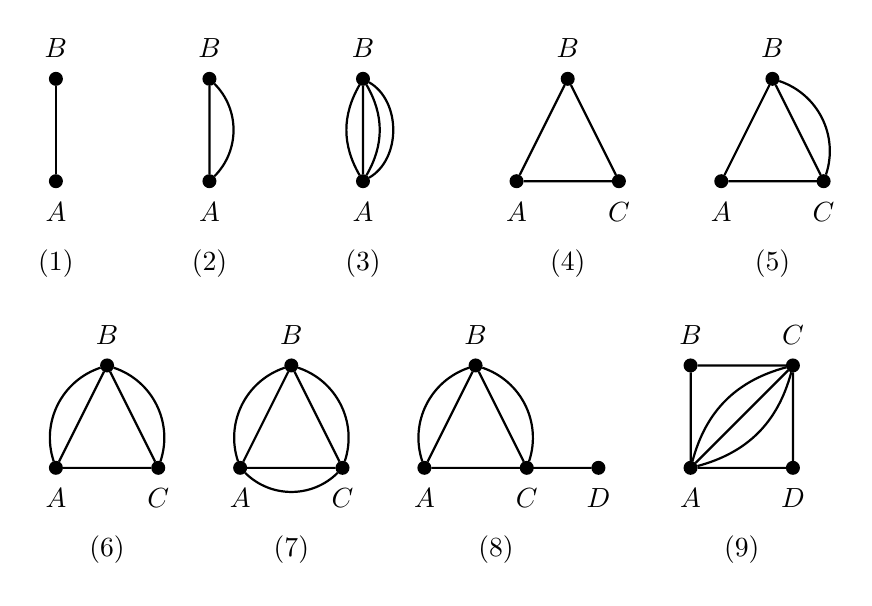
\begin{tikzpicture}[scale=1.3, every node/.style={circle, draw=black, fill=black, inner sep=1.5pt}, every path/.style={thick}]

% --- Graph 1 ---
\node (a1) at (0,0) {};
\node (b1) at (0,1) {};
\draw (a1) -- (b1);
\node[draw=none, fill=none] at (0,-0.3) {$A$};
\node[draw=none, fill=none] at (0,1.3) {$B$};
\node[draw=none, fill=none] at (0,-0.8) {(1)};

% --- Graph 2 ---
\node (a2) at (1.5,0) {};
\node (b2) at (1.5,1) {};
\draw (a2) -- (b2);
\draw (a2) to[bend right=45] (b2);
\node[draw=none, fill=none] at (1.5,-0.3) {$A$};
\node[draw=none, fill=none] at (1.5,1.3) {$B$};
\node[draw=none, fill=none] at (1.5,-0.8) {(2)};

% --- Graph 3 ---
\node (a3) at (3,0) {};
\node (b3) at (3,1) {};
\draw (a3) -- (b3);
\draw (a3) to[bend left=30] (b3);
\draw (a3) to[bend right=30] (b3);
\draw (a3) to[bend right=60] (b3);
\node[draw=none, fill=none] at (3,-0.3) {$A$};
\node[draw=none, fill=none] at (3,1.3) {$B$};
\node[draw=none, fill=none] at (3,-0.8) {(3)};

% --- Graph 4 ---
\node (a4) at (4.5,0) {};
\node (c4) at (5.5,0) {};
\node (b4) at (5,1) {};
\draw (a4) -- (b4) -- (c4) -- (a4);
\node[draw=none, fill=none] at (4.5,-0.3) {$A$};
\node[draw=none, fill=none] at (5.5,-0.3) {$C$};
\node[draw=none, fill=none] at (5,1.3) {$B$};
\node[draw=none, fill=none] at (5,-0.8) {(4)};

% --- Graph 5 ---
\node (a5) at (6.5,0) {};
\node (c5) at (7.5,0) {};
\node (b5) at (7,1) {};
\draw (a5) -- (b5) -- (c5) -- (a5);
\draw (b5) to[bend left=45] (c5);
\node[draw=none, fill=none] at (6.5,-0.3) {$A$};
\node[draw=none, fill=none] at (7.5,-0.3) {$C$};
\node[draw=none, fill=none] at (7,1.3) {$B$};
\node[draw=none, fill=none] at (7,-0.8) {(5)};

% ===== Shifted lower row (was y=-2, now y=-2.8) =====

% --- Graph 6 ---
\node (a6) at (0,-2.8) {};
\node (c6) at (1,-2.8) {};
\node (b6) at (0.5,-1.8) {};
\draw (a6) -- (b6) -- (c6) -- (a6);
\draw (a6) to[bend left=45] (b6);
\draw (b6) to[bend left=45] (c6);
\node[draw=none, fill=none] at (0,-3.1) {$A$};
\node[draw=none, fill=none] at (1,-3.1) {$C$};
\node[draw=none, fill=none] at (0.5,-1.5) {$B$};
\node[draw=none, fill=none] at (0.5,-3.6) {(6)};

% --- Graph 7 ---
\node (a7) at (1.8,-2.8) {};
\node (c7) at (2.8,-2.8) {};
\node (b7) at (2.3,-1.8) {};
\draw (a7) -- (b7) -- (c7) -- (a7);
\draw (a7) to[bend right=45] (c7);
\draw (b7) to[bend left=45] (c7);
\draw (a7) to[bend left=45] (b7);
\node[draw=none, fill=none] at (1.8,-3.1) {$A$};
\node[draw=none, fill=none] at (2.8,-3.1) {$C$};
\node[draw=none, fill=none] at (2.3,-1.5) {$B$};
\node[draw=none, fill=none] at (2.3,-3.6) {(7)};

% --- Graph 8 ---
\node (a8) at (3.6,-2.8) {};
\node (c8) at (4.6,-2.8) {};
\node (d8) at (5.3,-2.8) {};
\node (b8) at (4.1,-1.8) {};
\draw (a8) -- (b8) -- (c8) -- (d8) -- (a8);
\draw (a8) to[bend left=45] (b8);
\draw (b8) to[bend left=45] (c8);
\node[draw=none, fill=none] at (3.6,-3.1) {$A$};
\node[draw=none, fill=none] at (4.6,-3.1) {$C$};
\node[draw=none, fill=none] at (5.3,-3.1) {$D$};
\node[draw=none, fill=none] at (4.1,-1.5) {$B$};
\node[draw=none, fill=none] at (4.3,-3.6) {(8)};

% --- Graph 9 ---
\node (a9) at (6.2,-2.8) {};
\node (d9) at (7.2,-2.8) {};
\node (c9) at (7.2,-1.8) {};
\node (b9) at (6.2,-1.8) {};
\draw (a9) -- (b9) -- (c9) -- (d9) -- (a9) -- (c9);
\draw (a9) to[bend left=30] (c9);
\draw (a9) to[bend right=30] (c9);
\node[draw=none, fill=none] at (6.2,-3.1) {$A$};
\node[draw=none, fill=none] at (7.2,-3.1) {$D$};
\node[draw=none, fill=none] at (7.2,-1.5) {$C$};
\node[draw=none, fill=none] at (6.2,-1.5) {$B$};
\node[draw=none, fill=none] at (6.7,-3.6) {(9)};

\end{tikzpicture}
\end{frame}

\begin{frame}{Some more examples}
    \begin{figure}
        \centering
        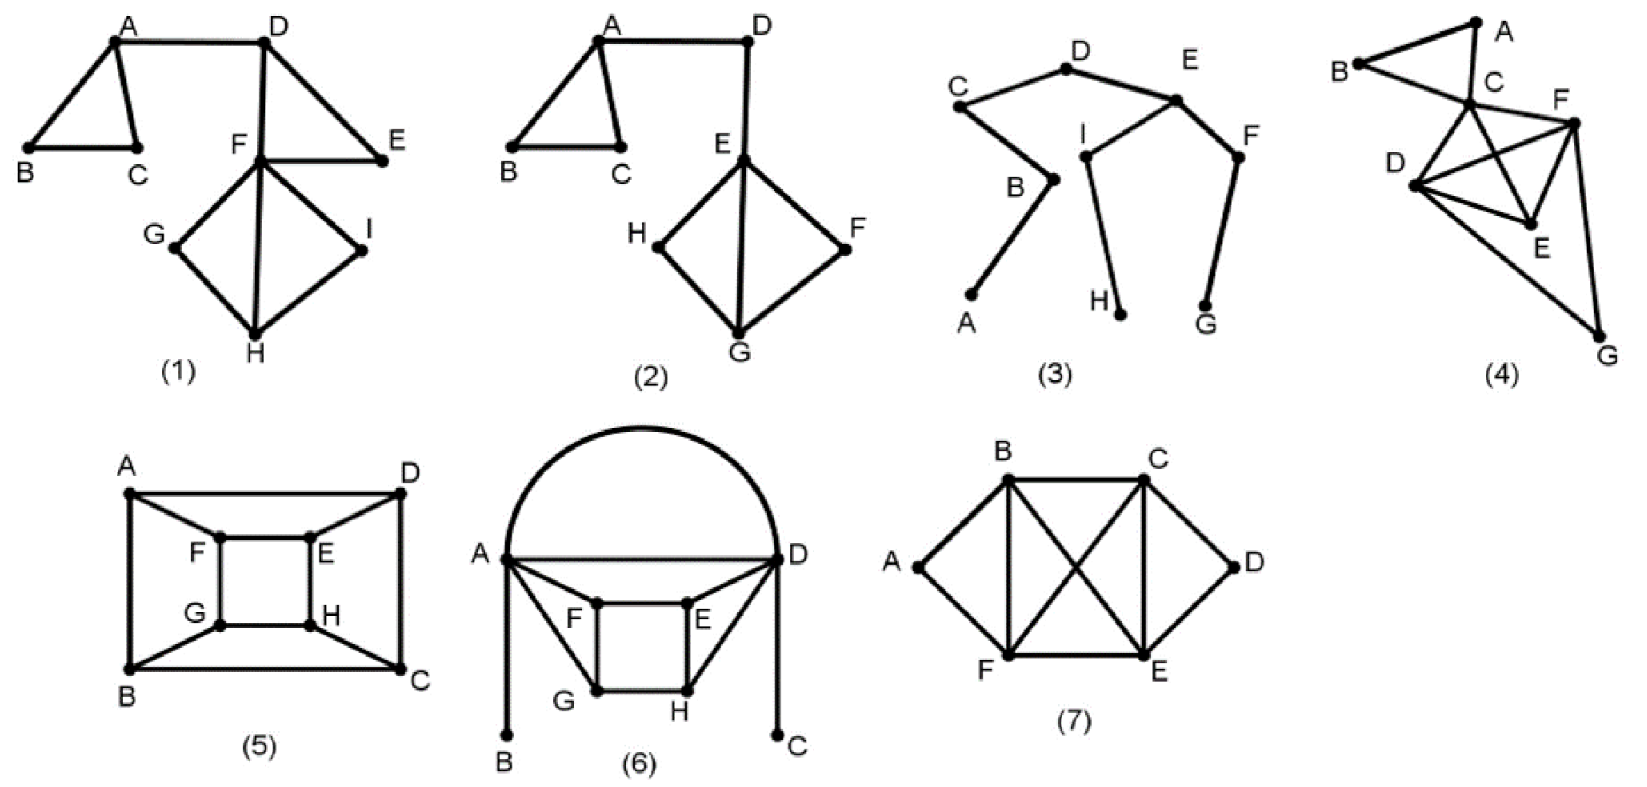
\includegraphics[width=\textwidth]{example2.png}
    \end{figure}
\end{frame}


\begin{frame}{Do you see any patterns?}
    \begin{itemize}
        \item Fill up the tables
        \item What feature of a graph makes it traceable?
        \item What pattern do you see for the graphs where the starting and ending point of the
    path is the same vertex?
    \item What about the graphs where starting and ending points are different? 
    \end{itemize}
\end{frame}

\begin{frame}{Observations}
% \begin{table}
%     \begin{tabular}{c|c} \hline
%         Position of node in the path & Degree \\ \hline
%         Node is both starting and final point & Even \\   
%         Node is starting point but not final point & Odd \\  
%         Node is final point but not starting point & Odd \\ 
%         Node is neither starting nor final point & Even \\ \hline
%     \end{tabular}
% \end{table}

An\textbf{ Eulerian path} is a trail in a finite graph which visits every edge exactly
once. Similarly, an \textbf{Eulerian cycle} is a Eulerian trail which starts and ends on the same vertex.
\pause
\begin{block}{Conditions}
    \begin{itemize}
        \item For an Eulerian path a graph must have two vertices with odd degrees.
        \item For an Eulerian cycle, a graph must have all even degree vertices. 
    \end{itemize}
\end{block}
\end{frame}

\begin{frame}{Euler enters!}
    \begin{figure}
        \centering
        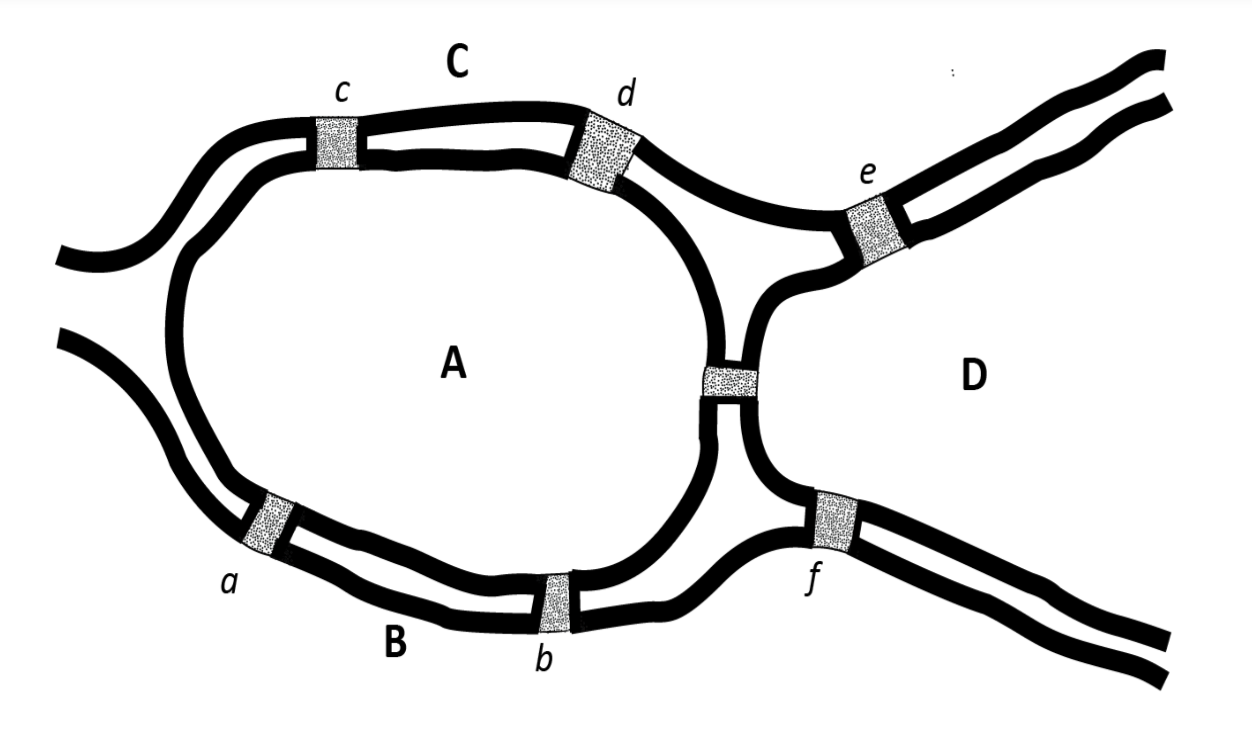
\includegraphics[scale=.25]{euler's map.png}
    \end{figure}
    Can you map this to the map we have seen?
\end{frame}

\begin{frame}{Try this out}
    \begin{figure}
        \centering
        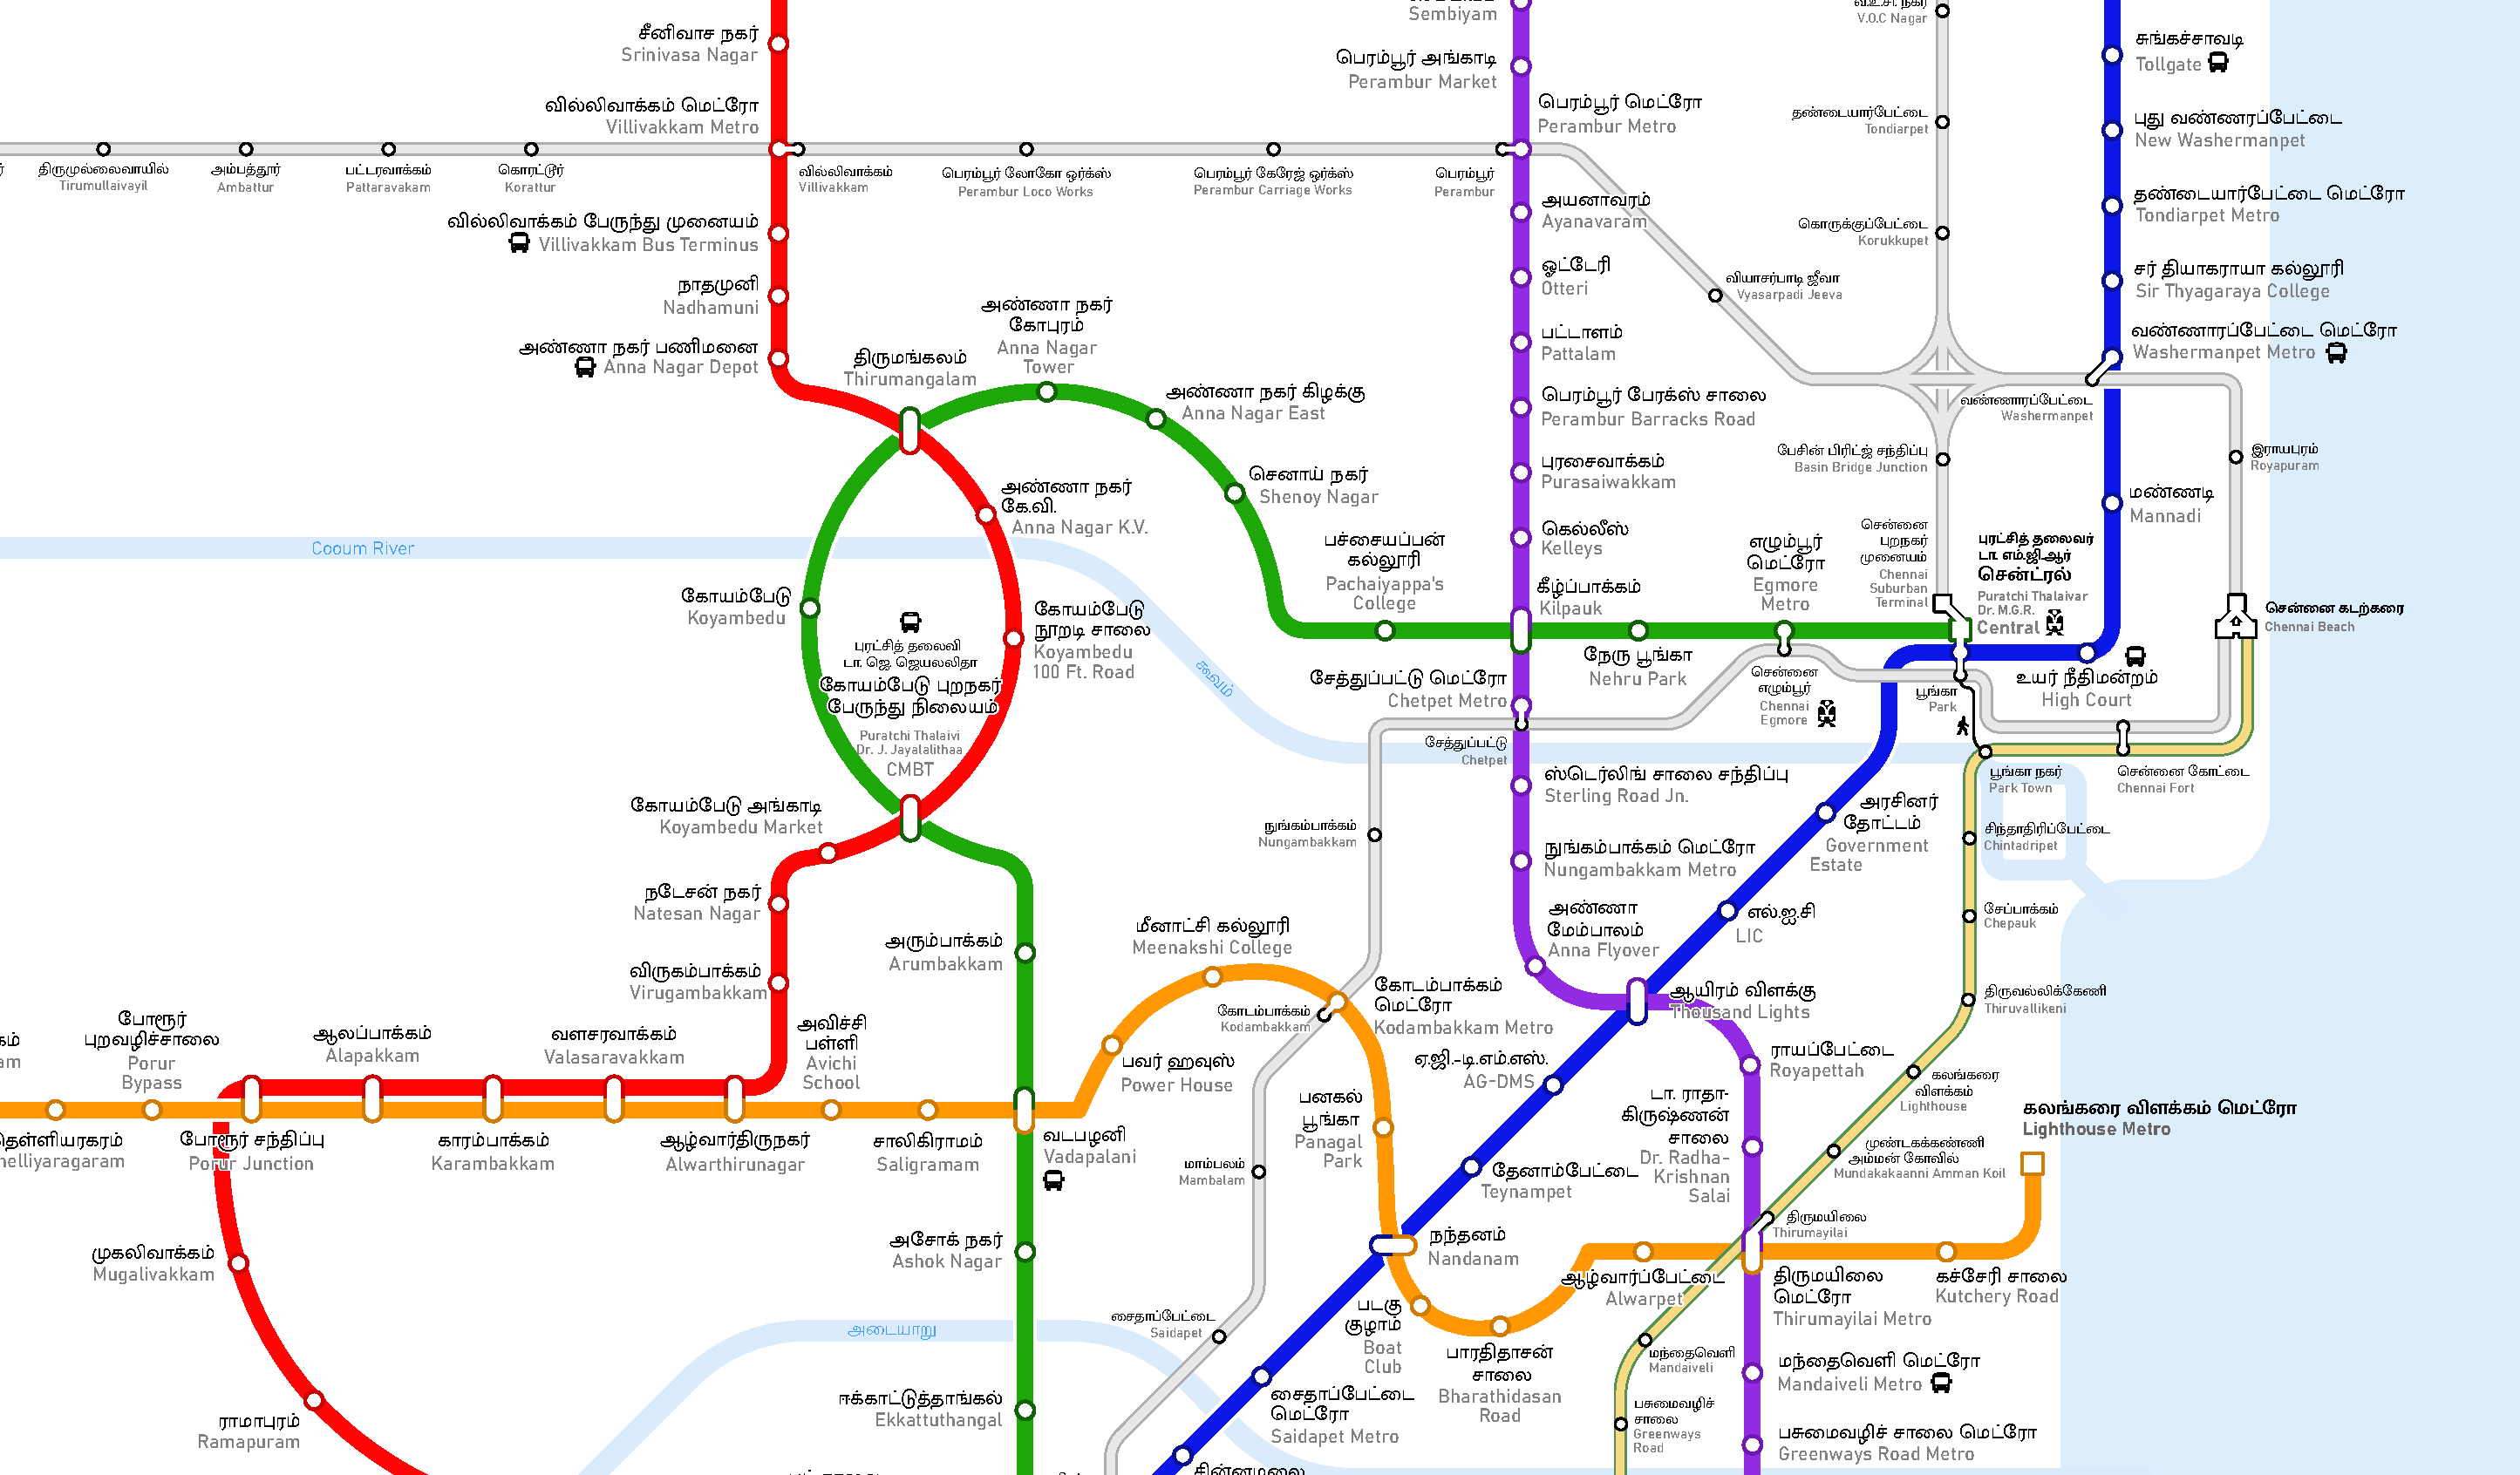
\includegraphics[width=\textwidth]{metromap_cropped.pdf}
    \end{figure}
\end{frame}


\begin{frame}{How to represent a graph}
    \begin{columns}

        %--- Graph on the Left ---
        \begin{column}{0.5\textwidth}
            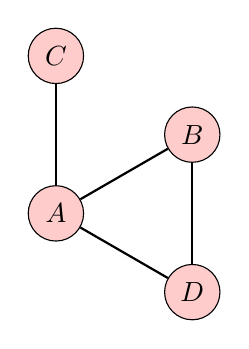
\begin{tikzpicture}[
                node style/.style={circle, draw=black, fill=red!20, minimum size=20pt, inner sep=2pt}
]

    % Center node A
        \node[node style] (A) at (0,0) {$A$};

    % Place B and D on a circle around A
        \node[node style] (B) at ([shift={(30:2cm)}]A) {$B$}; % 30° angle
        \node[node style] (D) at ([shift={(-30:2cm)}]A) {$D$}; % -30° angle
    % Node C remains at top manually
        \node[node style] (C) at (0,2) {$C$};
    % Edges
        \draw[thick] (A) -- (B);
        \draw[thick] (A) -- (C);
        \draw[thick] (A) -- (D);
        \draw[thick] (B) -- (D);
\end{tikzpicture}
        \end{column}

        %--- Adjacency Matrix on the Right ---
        \begin{column}{0.5\textwidth}
            \begin{block}{Adjacency Matrix}
            \[
            \begin{pmatrix}
                & A & B & C & D \\
                A & 0 & 1 & 1 & 1 \\
                B & 1 & 0 & 0 & 0 \\
                C & 1 & 0 & 0 & 0 \\
                D & 1 & 1 & 0 & 0 \\
            \end{pmatrix}
            \]
            \end{block}

            \begin{block}{Edge List}
                \begin{align*}
                    \{(A,B),(A,C),
                    (A,D),(B,D)\}
                \end{align*}
            \end{block}
        \end{column}
    \end{columns}
\end{frame}
\end{document}
